\section{Experimental Results}

\begin{figure*}[t!]
    \centering
    \begin{subfigure}[t]{0.5\textwidth}
        \centering
        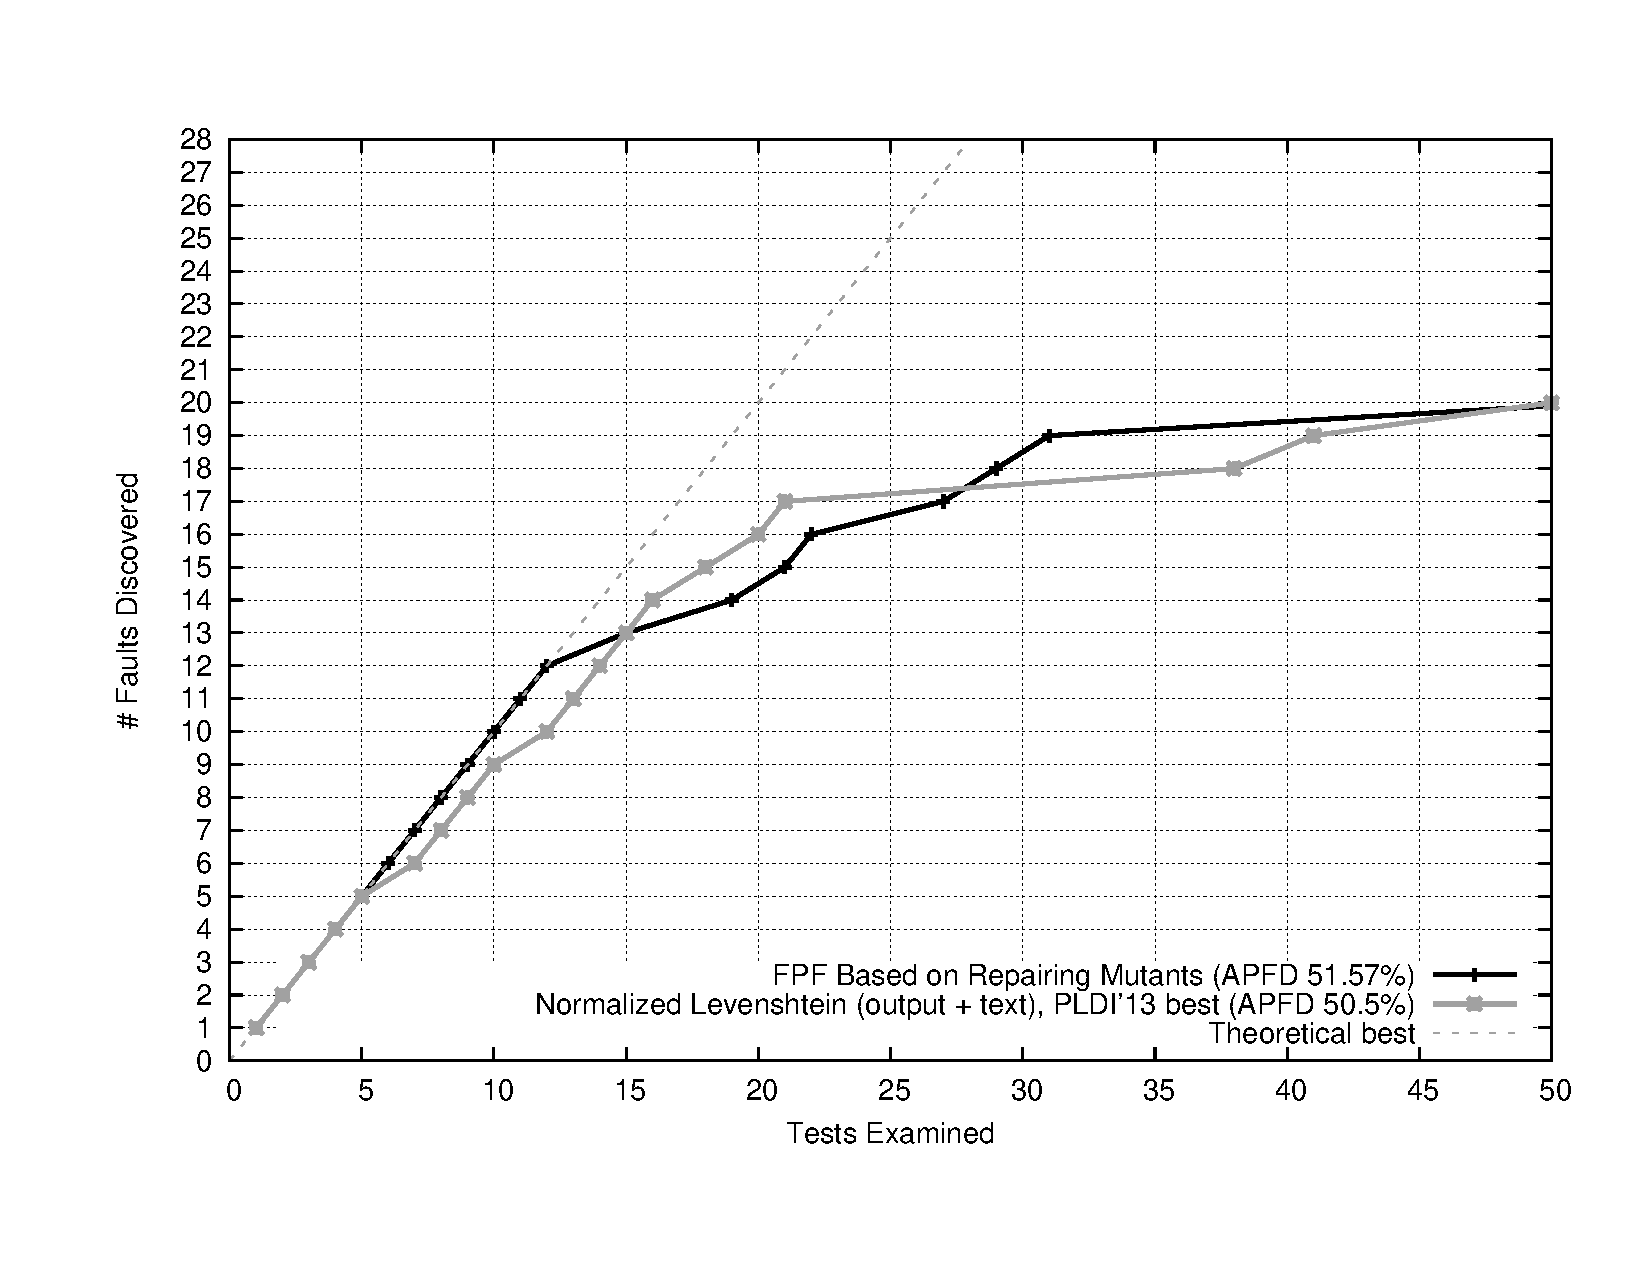
\includegraphics[width=1.0\textwidth]{jscurve}
        \caption{Discovery curves for SpiderMonkey 1.6 faults}
        \label{jscurves}
    \end{subfigure}%
    ~ 
    \begin{subfigure}[t]{0.5\textwidth}
        \centering
        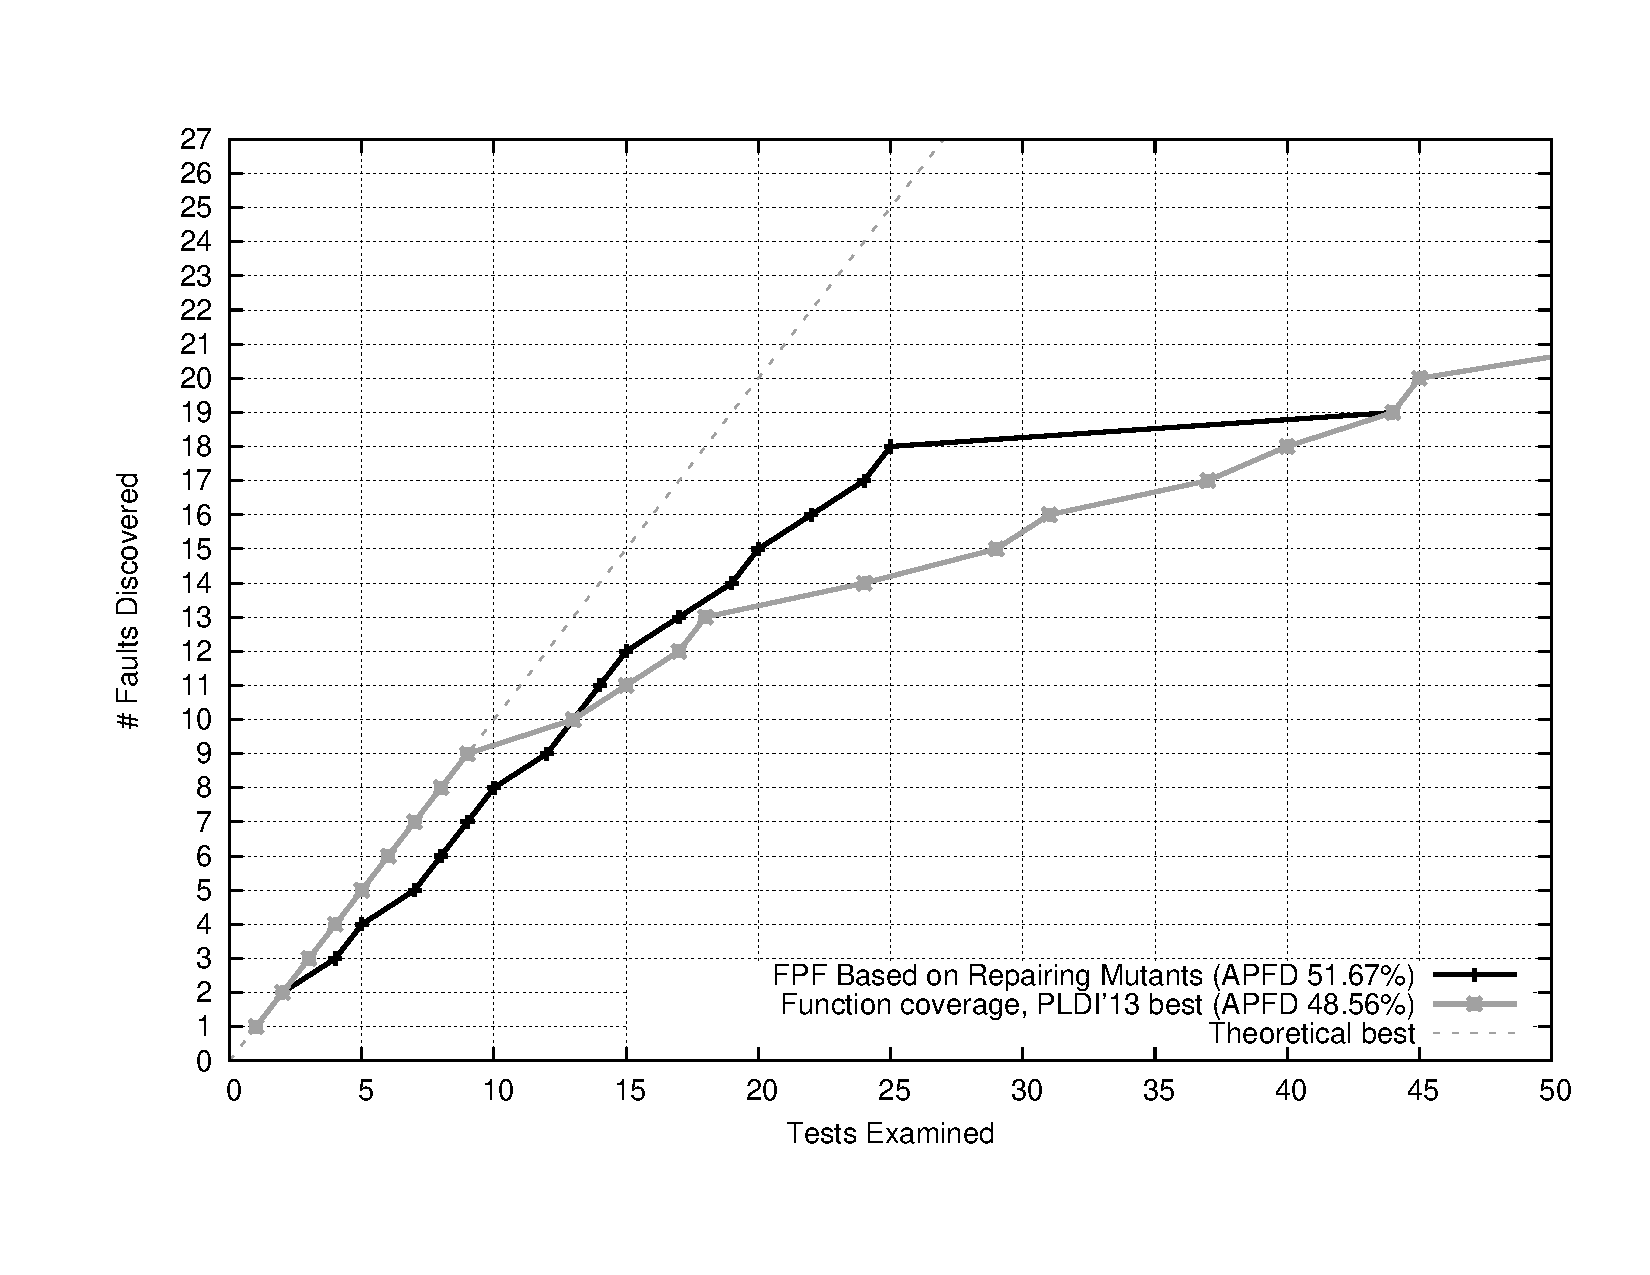
\includegraphics[width=1.0\textwidth]{gcccurve}
        \caption{Discovery curves for GCC 4.3.0 wrong-code faults}
        \label{gcccurves}
    \end{subfigure}
    \caption{Discovery curves compared to best curves from Chen et. al PLDI 2013 data (FPF benchmark)}
\end{figure*}


%\begin{figure*}
%\centering
%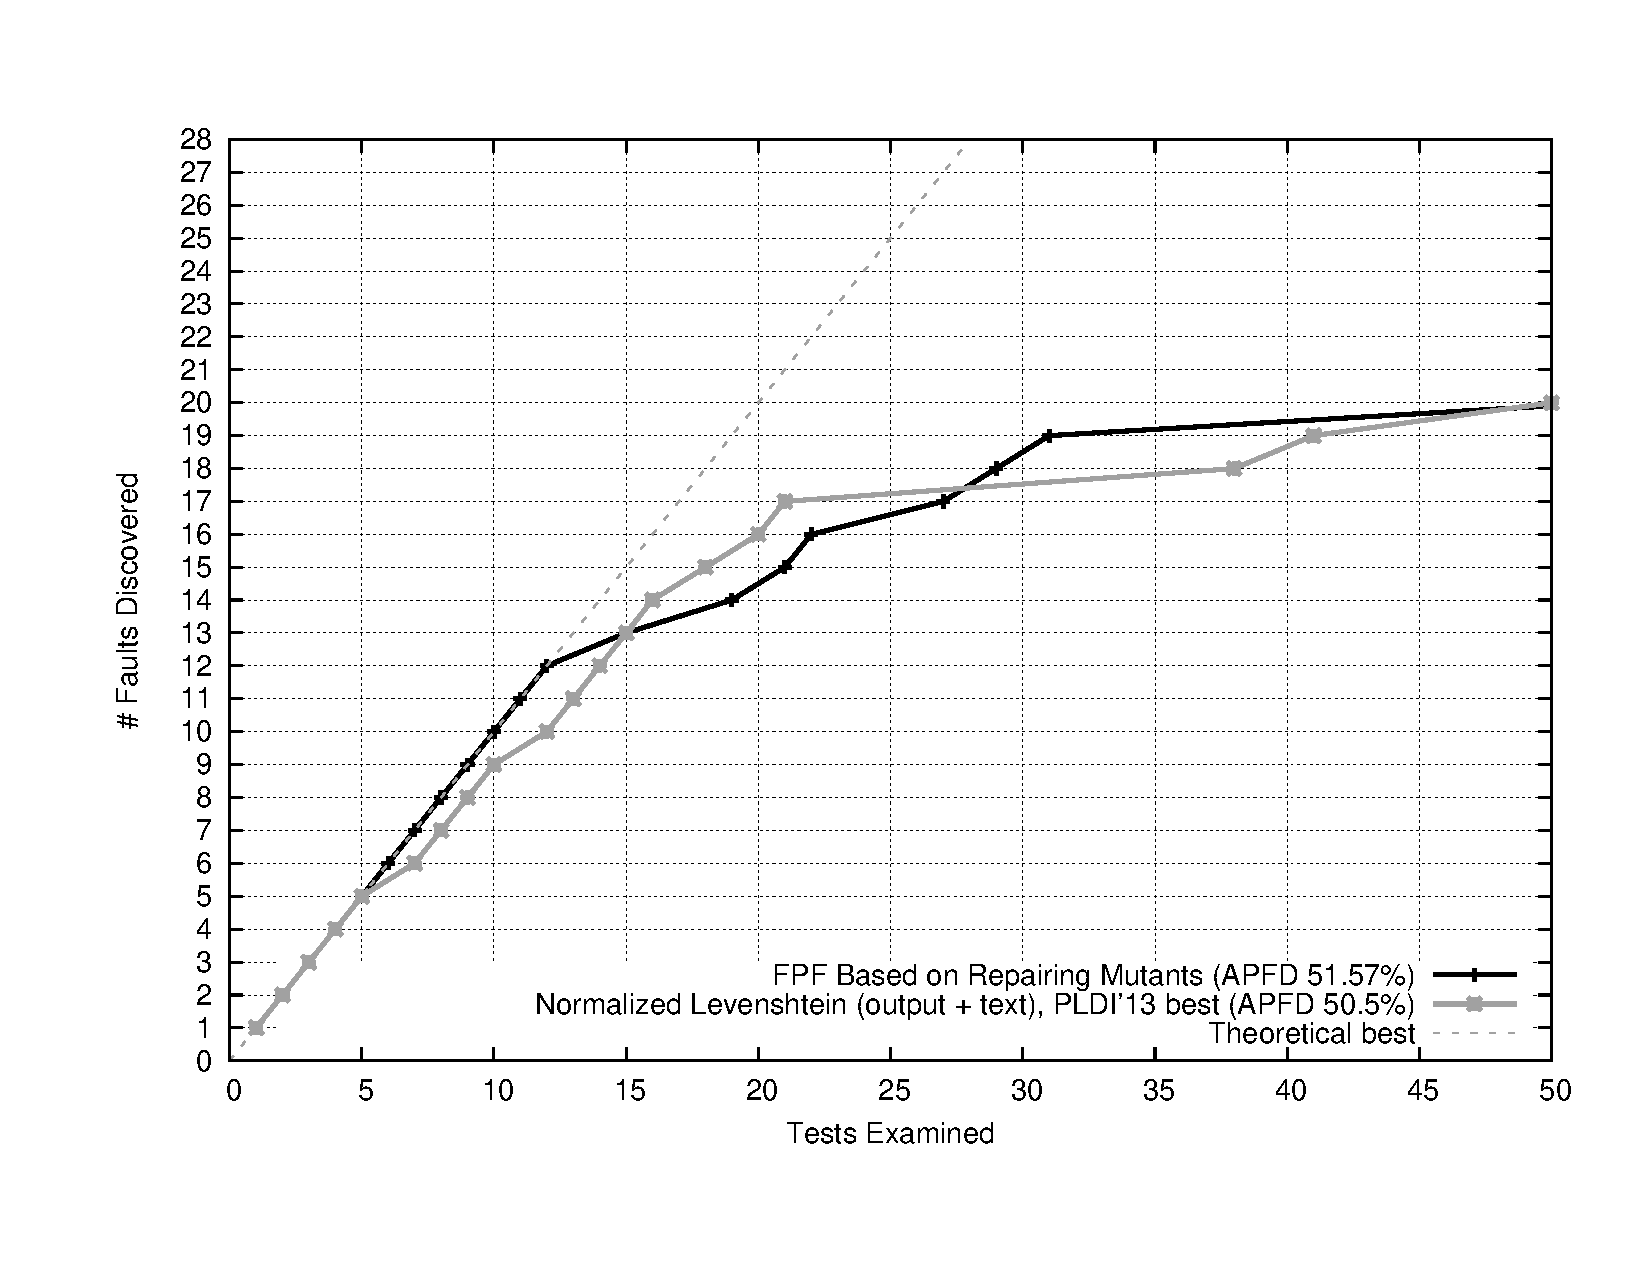
\includegraphics[width=2\columnwidth]{jscurve}
%\caption{Discovery curves for SpiderMonkey 1.6 faults}
%\label{jscurves}
%\end{figure*}


%\begin{figure*}
%\centering
%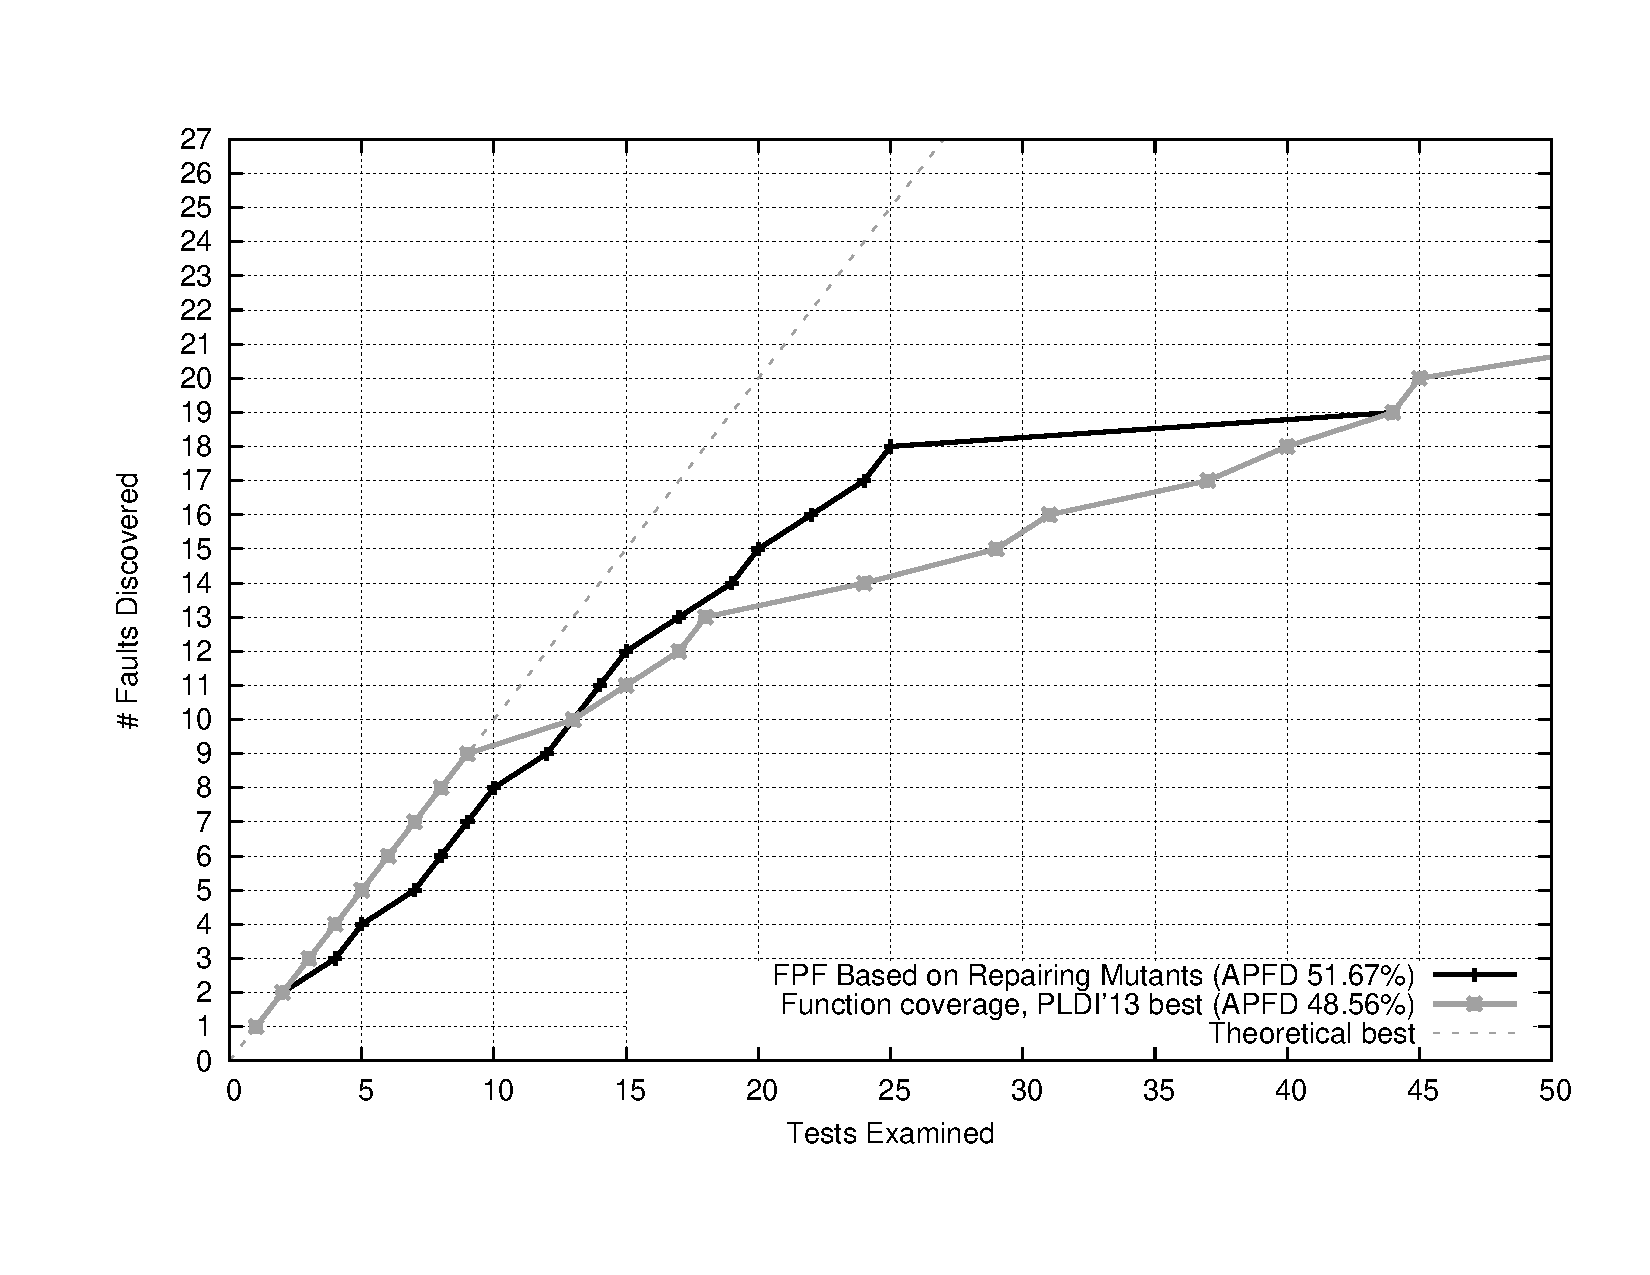
\includegraphics[width=2\columnwidth]{gcccurve}
%\caption{Discovery curves for GCC 4.3.0 wrong-code faults}
%\label{gcccurves}
%\end{figure*}

%\subsection{General Experimental Framework}

Our primary experiments are based on subjects used in the only previous study of compiler fuzzer taming (from Chen et al.'s PLDI 2013 paper \cite{PLDI13}), which we hereafter refer to as the FPF benchmark.  Of the three data sets examined in that paper, this paper considers two:  faults and tests cases for SpiderMonkey 1.6, Mozilla's JavaScript engine, with tests generated by {\tt jsfunfuzz} \cite{jsfunfuzz}, and \emph{wrong code} faults and test cases for GCC 4.3.0, with tests generated by Csmith \cite{csmith}.  GCC 4.3.0 crash faults were essentially perfectly localized by previous approaches.  In fact, on examination, only two of the 11 crash bugs are not distinguished by simply examining the crash message.  Faults that produce a crash are also likely to be much easier to debug than semantic problems such as all of the GCC wrong code bugs and most of the JavaScript faults --- e.g., following a dynamic slice might well suffice.

\comment{
We applied our metric to two of the datasets used in the previous study of compiler fuzzer taming \cite{PLDI13}: faults and tests cases for SpiderMonkey 1.6, Mozilla's JavaScript engine, with tests generated by {\tt jsfunfuzz} \cite{jsfunfuzz}, and \emph{wrong code} faults and test cases for GCC 4.3.0, with tests generated by Csmith \cite{csmith}.   We did not use the crash faults from that data set, as these are in practice fairly easy to identify by hand (and perfectly identified by previous metrics), and also typically easy to debug.  }

Our mutants were produced using the tool written by Jamie Andrews \cite{mutant}.  Andrews' tool applies only four operators: statement deletion, conditional negation, operator replacement, and constant replacement, chosen as a small set that still produces good results for C code.  Experiments were performed on a MacBook Pro with 16GB RAM and dual-core 3.1GHz Intel Core i7; GCC executed on a VirtualBox-hosted Ubuntu 11.04.  For GCC, some test cases from the FPF set no longer failed, presumably due to unknown differences in execution environment, OS, or memory layout. Discarding these reduced the set of test cases from 1,275 to 1,117 and the number of distinct faults to 27 rather than 35.  For SpiderMonkey, all 1,749 test cases from the FPF benchmark failed in the new environment, representing 28 distinct faults.

These data sets, though similar in that both compilers are written in C, provide some interesting variance for testing our metrics.  The oracle for SpiderMonkey executions is the set of checks built in to {\tt jsfunfuzz} plus the requirement that the execution not crash.  This is only a moderately strong oracle, and allows serious deviations from both the JavaScript language specification and normal SpiderMonkey behavior, while checking some complex details, such as {\tt eval} round-trips.  For GCC, the oracle is a differential check on a hash code:  failure was defined as producing a executable with the -O3 flag that, when executed, produced a different checksum than code compiled by either of GCC 4.9.3 or clang 7.0.0, both using -O0.  A repairing mutant must enable GCC 4.3.0 to actually compile code correctly, which is a very strict correctness property, making coincidental correctness \cite{CCT} highly unlikely --- only missed optimizations are allowed.

We only show results for the first 50 tests in the ranking, and computed areas under curves for the same limit, since it seems very unlikely that a user will examine many more than 50 tests, especially given the decreasing slope of the discovery curves.  In practice, after 50 tests, fixing a few faults and then re-running tests and FPF seems the most likely recourse, and we confirmed that after removing random subsets of faults, our metrics still outperform the previous best.  We applied X-means \cite{xmeans} in an attempt to use clustering with our metrics, but, as with previous results \cite{PLDI13} it did not compare well with FPF, and the runtime was much higher.  We confirm the conclusion \cite{PLDI13} that clustering is of limited value in fuzzer taming.
% (at least with X-means) does not work well in a setting with extreme disparity in instance counts for faults.  %A further difficulty for our setting is that X-means and most off-the-shelf clustering tools take vectors, not a distance metric.  X-means is using the raw repair data, not weighted by the fact that 0-0 agreement is much less informative than other possible matchings (a Euclidean over 0-1 vectors is just the square root of Hamming distance).

\subsection{Mozilla SpiderMonkey 1.6 Results}


There were 96,828 SpiderMonkey mutants, based on 69,634 lines of code in C and header files.  Of these mutants, 12,666 were covered by some failing test case.  Of these mutants, 10,525 survived a basic set of SpiderMonkey quick tests \cite{icst2014}.  Of these mutants, 1,326 (12.6\%) repaired at least one test case.  Figure \ref{jscurves} shows the discovery curves for the mutant repair metric compared to the ideal discovery curve and the best curve from previous work using FPF, which used a normalized Levenshtein distance \cite{lev} over the failure output and test case text \cite{PLDI13}.  A discovery curve is a plot of the number of distinct faults that a user, examining the tests in the ranked order, would have seen after N tests (here, N goes up to 50).

The APFD (Average Percent Faults Detected) values in the graphs are based on the measure  introduced by Rothermel et al. for evaluating test case prioritization methods \cite{APFD}.  APFD is a somewhat better summary of results than the raw curve areas used for evaluation in previous work \cite{PLDI13}.  APFD, as the name suggests, measures the percent of all faults discovered at the ``average'' point on the curve, by comparing the curve's area to an ideal curve, with interpolation.  A simpler (but less informative) way to compare the curves is to note that the mutation-based metric's curve is above the best previous curve at 60\% of data points.
%\footnote{The details of APFD calculation are slightly involved, and the interpolation and perfect curve are not exact fits for fuzzer taming; nonetheless the basic method summarizes curves fairly well and is standard in the testing literature for similar problems \cite{issta14}.}. 

APFD results are useful summaries, but the curve itself is also worth examining, since (1) long sequences of tests with no new faults may discourage users more than an overall less effective but steadily climbing curve with few ``plateaus'' as we call these uninformative sequences of tests and (2) a good early curve is important to developers.  The mutant repair curve climbs very rapidly in the early portion, with perfect discovery for the first 12 faults. The largest plateau is 5 tests without a new fault, ignoring the long period after the 31st test.  In fact, a plateau at the end of the curve is not problematic.  Assuming that few users will examine more than 50 test cases without fixing some faults, the user may give up after seeing 10 or more tests without a new fault based on the mutant repair curve, and in fact lose nothing by doing so.  The best FPF benchmark curve, in contrast, has a plateau of size 17 after the 17th fault.  If we assume a user stops examining tests after a size 10 or greater plateau, the user will only see 17 faults using the best benchmark metric, vs. 19 with our metric.  Stopping at a plateau of size 6 produces the same results.

Over all mutants, and all pairs of test cases repaired by the same mutant (so the same pair may count many times, if many mutants repair both test cases), the probability of being due to the same fault was 42.77\%, and the probability of being due to the same fault if two test cases disagreed on a repair (the mutant repaired one test case but not the other) was only 20.33\%.  The baseline rate for same-fault for test pairs was 33.64\%.  Just knowing that two test cases have \emph{one} shared repairing mutant makes it 1.27x more likely that they are the same fault, and knowing they differ for one mutant makes it 0.6 times as likely they are due to the same fault.  Matching non-repair, however, provides very weak evidence:  only a 34.14\% chance of matching fault, just over baseline.

An additional measure of effectiveness is to consider how effective a metric is in producing matched nearest neighbors.  That is, how often is the nearest neighbor of a failure (that is not due to a singleton fault --- a fault detected by only one test case) due to the same fault?  For reduced \cite{DD,PLDI13,
CReduce} test cases, we assume that for a perfect metric, the nearest neighbor should almost always share the same fault, since there is little or no extraneous semantic content to each test beyond the cause of failure.  For the SpiderMonkey failures, 96.3\% of non-singleton failures matched their nearest neighbor(s).  For mutants that repaired any failures, the mean and median number of test cases repaired were 120.6 and 4.0, respectively.  Most mutants repaired a small number of tests, but a few mutants repaired a very large number of tests.  A few mutants repaired \emph{all} SpiderMonkey faults; obviously these mutants were not actual fault fixes, but effectively disabled the mechanism {\tt jsfunfuzz} used to detect failure. The mean and median homogeneity for repairing mutants (\% of failures repaired corresponding to the most common fault repaired) were 77.96\% and 86.36\%, respectively.  

In order to check our results statistically, we sliced the FPF benchmark tests into 20 randomly selected equal-sized (as much as possible) distinct subsets.  The repair metric had a mean APFD (89.23\%) for these subsets that was 2.85\% better than the mean APFD for the best benchmark metric (86.76\%), over sets of $\sim 10$ faults. The result was statistically significant ($p < 0.05$ by Wilcoxon test).   Median repair APFD was 90.05\%, vs. 84.75\% for the best benchmark metric.


\subsubsection{Fault Localization}

Table \ref{bothtable} shows a comparison of three fault localization methods for the SpiderMonkey (and GCC) faults.  The first column is a fault ID. The next three columns show localization rankings.  A dash for a column means that localization did not rank any faulty statements, or assigned all faulty statements suspiciousness of 0.0.  The three rankings are: our {\bf Repair} localization, the MUSE \cite{MUSE} localization, and the MUSEUM \cite{multilingual} localization.  MUSEUM uses the same formula as MUSE, but works better for multiple faults because it uses only one failure.  The MUSE/MUSEUM formulas normally make use of information from passing tests as well: when mutating a statement makes a passing test case fail, it makes the statement \emph{less} suspicious, by a weighted amount. The weight assigned to information from passing tests in our setting would likely be low (due to the ratios of repairs to mutation kills).  In a limited sense, information from passing tests is already incorporated in our results.  Throwing out all mutants that are killed by any passing test as potential repairs/localizations ensures that the rankings of all statements that are in MUSE/MUSEUM rankings are correct, \emph{relative to each other}.  By definition, passing tests have no influence on the suspiciousness of these mutants.  However, there may be other mutants that 1) repair a failure and 2) are killed by some test case: these could, if enough different ones repaired the same faulty statement, improve MUSE/MUSEUM results, though in practice this is extremely unlikely.  We reject such mutants in part to keep costs low, and in part because we think that the causal information contained in such mutants, that ``fix'' a failure but also break some passing test(s), is problematic.  They seem likely to be less useful as explanations of the causes of a failure, since they do not impact the program semantics in a way that is only known to be beneficial, and could potentially even mislead a user if used as explanations.  \comment{Still, it is most useful to compare MUSEUM/MUSE and our approach on the cases where all methods produce a localization.}

Discussion with the MUSE/MUSEUM authors confirms  that adding information for passing tests, while costly, would likely improve the MUSE and MUSEUM results, given the weakness of our oracles, particularly for SpiderMonkey, and should be considered essential for ideal application of their approach.  Because the cost of recording the full mutant analysis matrix for all passing tests (rather than considering a mutant killed as soon as one test fails, as we do) is very high, and we would like to produce a comparison over a fixed computational cost, we give results for MUSE/MUSEUM over failing tests only, cautioning that we are not sure what the impact of this choice is on faults that were not localized.  For similar reasons of keeping costs low, we also used the mutation operators of Andrews vs. the more extensive Proteum \cite{Proteum} operators used in MUSE/MUSEUM's evaluations.  \comment{Even with these restrictions, running all mutants on passing tests until at least a single kill was observed took about 3 times as long as the search for repairs, which we already consider a potentially problematic cost.}  In Section \ref{sec:otherfaults} we provide some comparisons with MUSEUM and MUSE fault localization in the context of a full mutation result matrix using their preferred set of operators.

\comment{
Results are reported as absolute ranks, rather than more sophisticated \cite{MUSE} localization evaluations because our localizations do not assign suspiciousness scores, only rankings, and in accord with the proposal of Parnin and Orso that only localizations ranking a fault in the top few statements may be useful to users \cite{AutoHelp}.  We expect users to examine coverage changes and mutants.  Blind, unaided pointers to portions of compiler code without more semantic information about why the statement is suspicious seem unlikely to work well, based on our experience with complex compiler faults, and the results of Parnin and Orso \cite{AutoHelp}.
}

\comment{
\begin{table}
\centering
{\scriptsize
\begin{tabular}{|c||c|c|c|}
\hline
%& \multicolumn{3}{|c|}{Localization Rank} \\
%\hline
Fault & Repair & MUSE & MUSEUM \\
\hline
880 & - & - & - \\
95 & - & 173 & -\\
1294 & 1 & 22 & 4 \\
60 & - & - & -\\
1543 & 19 & 118 & 26\\
1172 & 28 & 87 & 23\\
1561 & - & - & - \\
115 & 3 & 133 & 5 \\
\hline
\end{tabular}
}
\caption{Fault localization results for SpiderMonkey}
%\vspace{-0.2in}
\label{jstable}
\end{table}
}

%%%%%%%%%%%%%%%%%%%%%%%%%%%%%%%%%%%%%%%%%%%%%%%%%%%%%%%%%%%%%%%%%
% \begin{comment}                                               %
% \begin{figure}                                                %
% {\scriptsize                                                  %
% \begin{code}                                                  %
% {\bf Diff of old ($<$) vs new ($>$) for 115 patch (portion):} %
% ...                                                           %
% <             vp[1] = OBJECT\_TO\_JSVAL(thisp);               %
% <         \} else \{                                          %
% <             ok = OBJ\_GET\_PROPERTY(cx, thisp, id, \&v);    %
% <         \}                                                  %
% ...                                                           %
% <                   a->avail = (jsuword)sp;                   %
% <               \}                                            %
% ...                                                           %
% ---                                                           %
% >         RESTORE\_SP(fp);                                    %
% ...                                                           %
% {\bf Mutant information:}                                     %
% Failure repaired by 148 mutants.                              %
% ...                                                           %
% \#3: delete statement mutant of jsinterp.c:944:               %
%                                                               %
%             vp[1] = OBJECT\_TO\_JSVAL(thisp);                 %
%         \} else \{                                            %
% /*MUTANT    ok = OBJ\_GET\_PROPERTY(cx, thisp, id, \&v);*/    %
%         \}                                                    %
%                                                               %
% {\bf Coverage change information:}                            %
% ...                                                           %
% \#6: 5 mutants (3.38\% of repairs) added jsinterp.c:992:      %
%                    a->avail = (jsuword)sp; /* ADDED */        %
% \end{code}                                                    %
% }                                                             %
% \caption{Patch and explanation for fault 115}                 %
% %\vspace{-0.18in}                                             %
% \label{fig:explain}                                           %
% \end{figure}                                                  %
% \end{comment}                                                 %
%%%%%%%%%%%%%%%%%%%%%%%%%%%%%%%%%%%%%%%%%%%%%%%%%%%%%%%%%%%%%%%%%

Table \ref{bothtable} only includes 8 of the 28 SpiderMonkey faults.  This is due to a problem with the data set:  producing ground truth patches for a large application, in the sense of finding a minimal, clearly fault-fixing code change that can be back-ported to the original code is difficult \cite{PLDI13}.  While we believe the 28 faults identified in the FPF benchmark data are correct, it is very difficult to produce a valid patch of version 1.6 that captures the fix for most of these faults.  In some cases the final commit that caused tests to stop failing appeared to only be the end of a complex series of changes that converged on a correct fix.  In other cases, the code was modified so extensively before the fix that identifying ``the incorrect part'' of the original code seemed to owe more to guesswork than certainty.  The evaluation of localization therefore only examines the 8 faults for which we could be reasonably certain that the patch to 1.6 was correct and characterized the fault in question accurately.  In no case was the patch equivalent to one of the mutants (the smallest patch modified two statements).

No method performs extremely well --- for half the faults, no methods produced what we consider a useful localization.   Compiler faults are hard to debug, and any help is useful, but it seems unlikely developers will really benefit from a localization when it does not rank at least one faulty statement in the first 25-30 statements.  By this measure, MUSE only provides a helpful localization once, and performs worst of the methods.  {\bf Repair} and MUSEUM both perform well, with {\bf Repair} slightly better.

%%%%%%%%%%%%%%%%%%%%%%%%%%%%%%%%%%%%%%%%%%%%%%%%%%%%%%%%%%%%%%%%%%%%%%%%%%%%%%%%%%%%%%%%%%%%%%%%%%%%%%%%%%%%%%%%%%%%%%%%%%%%%%%%%%%%%%%%%%%%%%%%%%%%%%%%%%%%%%%%%%%%%%%%%%%%%%%%%%%%%%%%%%%%%%%%%%%%%%%%%%%%%%%%%%%%%%%%%%%%%%%%%%%%%%%%%%%%%%%%%%%%%%%%%%%%%%%%%%%%%%%%%%%%%%%%%%%%%%%%%%%%%%%%%%%%%%%%%%%%%%%%%%%%%%%%%%%%%%%%%%%%%%%%%%%%%%%%%%%%%%%%%%%%%%%%%%%%%%%%%%%%%%%%%%%%%%%%%%%%%%%%%%%%%%%%%%%%%%%%%%%%%%%%%%%%%%%%%%%%%%%%%%%%%%%%%%%%%%%%%%%%%%%%%%%%%%%%%%%%%%%%%%%%%%%%%%%%%%%%%%%%%%%%%%%%%%%%%%%%%%%%%%%%%%%%%%%%%%%%%%%%%%%%%%%%%%%%%%
% \begin{comment}                                                                                                                                                                                                                                                                                                                                                                                                                                                                                                                                        %
% \subsubsection{Error Explanation}                                                                                                                                                                                                                                                                                                                                                                                                                                                                                                                      %
%                                                                                                                                                                                                                                                                                                                                                                                                                                                                                                                                                        %
%                                                                                                                                                                                                                                                                                                                                                                                                                                                                                                                                                        %
% Figure \ref{fig:explain} shows part of the patch for SpiderMonkey fault 115, and the {\bf Coverage} and {\bf Repair} outputs that successfully localize the fault (the 6th coverage change output, and the 3rd mutant output), to give some idea of the information our methods present.  For {\bf Coverage}, it is surprising that the sixth highest ranked change only appeared in 5 of 148 repairs. This change ranked high out of thousands of changes because it was unusual, appearing for only 10 repairs in the entire SpiderMonkey analysis.  %
%                                                                                                                                                                                                                                                                                                                                                                                                                                                                                                                                                        %
% The precise form an explanation based on our techniques should take is not clear.  One possibility, suggested by the results here, is a method focused on repairs, but using common coverage changes.  For each repairing mutant, in rank order, the highest ranking coverage changes for that mutant could also be shown, to give an idea of unusual (and potentially localizing) changes induced by repair.                                                                                                                                          %
% \end{comment}                                                                                                                                                                                                                                                                                                                                                                                                                                                                                                                                          %
%%%%%%%%%%%%%%%%%%%%%%%%%%%%%%%%%%%%%%%%%%%%%%%%%%%%%%%%%%%%%%%%%%%%%%%%%%%%%%%%%%%%%%%%%%%%%%%%%%%%%%%%%%%%%%%%%%%%%%%%%%%%%%%%%%%%%%%%%%%%%%%%%%%%%%%%%%%%%%%%%%%%%%%%%%%%%%%%%%%%%%%%%%%%%%%%%%%%%%%%%%%%%%%%%%%%%%%%%%%%%%%%%%%%%%%%%%%%%%%%%%%%%%%%%%%%%%%%%%%%%%%%%%%%%%%%%%%%%%%%%%%%%%%%%%%%%%%%%%%%%%%%%%%%%%%%%%%%%%%%%%%%%%%%%%%%%%%%%%%%%%%%%%%%%%%%%%%%%%%%%%%%%%%%%%%%%%%%%%%%%%%%%%%%%%%%%%%%%%%%%%%%%%%%%%%%%%%%%%%%%%%%%%%%%%%%%%%%%%%%%%%%%%%%%%%%%%%%%%%%%%%%%%%%%%%%%%%%%%%%%%%%%%%%%%%%%%%%%%%%%%%%%%%%%%%%%%%%%%%%%%%%%%%%%%%%%%%%%%


\subsection{GCC 4.3.0 Wrong Code Results}


\begin{figure}
  \centering
  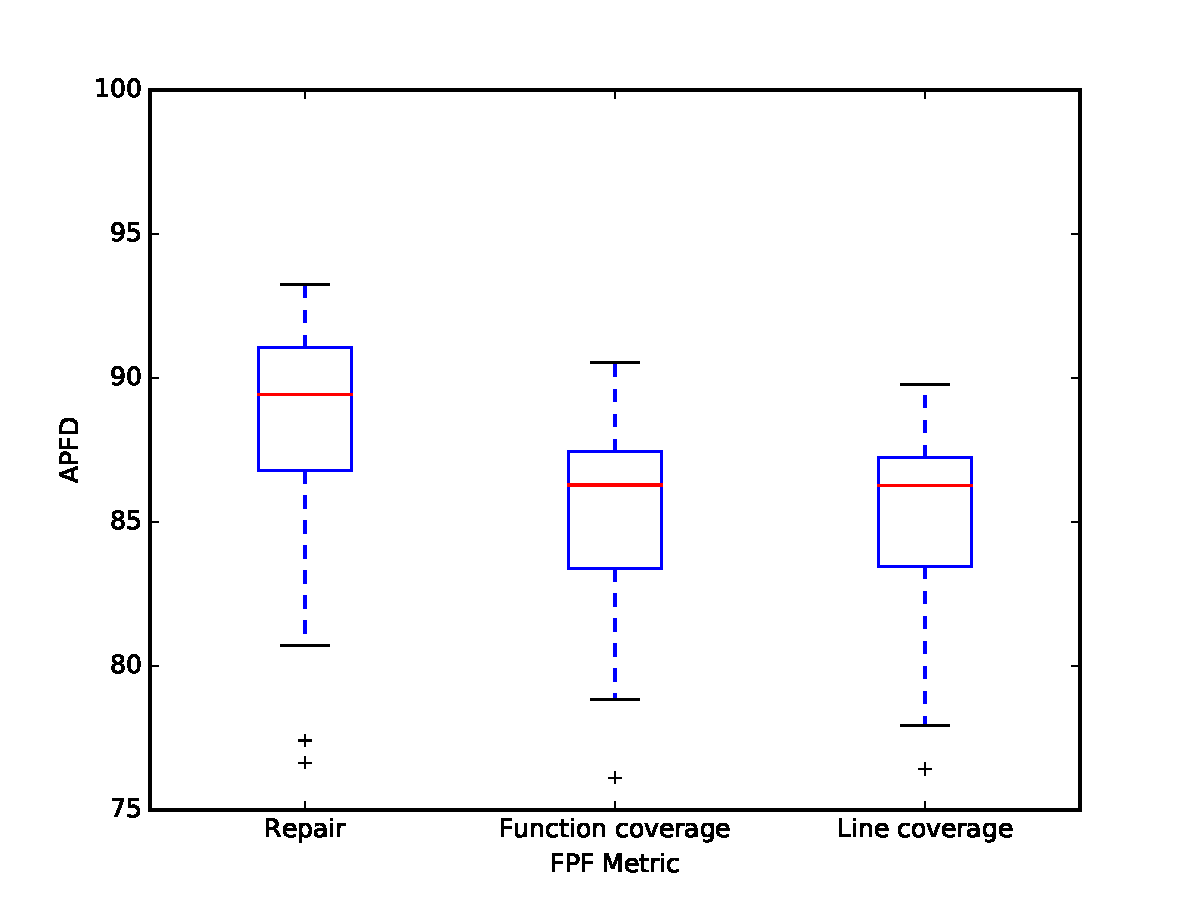
\includegraphics[width=0.8\columnwidth]{comparegcc}
  \caption{APFD values for GCC suite slices}
  \label{comparegcc}
\end{figure}%

There were 377,679 GCC mutants, based on 424,186 lines of code in C and header files. Of these mutants, 73,016 were covered by some failing test case.  Of these mutants, 41,385 survived a GCC bootstrap build, compiled hello world, and passed a GCC test suite.  Of these mutants, 3,232 (7.8\%) repaired at least one test case.  Figure \ref{gcccurves} shows discovery curves for the mutant repair metric vs. the best benchmark curve, Euclidean distance over function coverage vectors \cite{PLDI13}.  GCC's APFD improvement is larger than that for SpiderMonkey, but its early curve (first 15 tests) is worse compared to the benchmark curve, but still has a maximum gap of only 2 redundant tests vs. 4 for the benchmark.  Over all, again the curve is better than the best benchmark curve at 60\% of all points.  Using the hypothetical model where a user stops examining tests after a plateau of size 10, the user of the mutant-based taming will see 18 distinct faults by examining 25 tests, and the user of the function coverage based taming will see 20 faults after examining 45 tests.  If a user gives up after a plateau of size 5, our approach again lets a user examine 18 faults over 25 tests.  Function coverage only yields 16 faults over 31 tests. 


For GCC wrong code faults, the baseline chance that two test cases shared an underlying fault was 38.97\%.  Knowing that two test cases shared a repairing mutant raised the chance to 68.5\%, and knowing they disagreed on a repair lowered it to only 19.01\%.  The respective increase and decrease in probability of matching fault compared to baseline was thus 1.75 times greater for matching repairs, and less than 0.5 the chance of being the same fault, given one mismatched repair.  Knowing two test cases were both not fixed by a mutant again provided marginal evidence of sharing a fault: 39.2\% chance of matching faults.
For 99.3\% (all but 8) of the 1,090 non-singleton fault failures in GCC wrong code, the closest test case(s) by the repair metric showed the same fault.  The best previous reported FPF metric, function coverage vectors, had a matching rate of 92.2\%.   The mean and median numbers of repaired tests per mutant (for mutants that repaired any tests at all) were 18.4 and 3.0, respectively.  A few mutants fixed a very large number of tests, up to 1,050.  These all appear to be turning off all optimizations --- essentially running gcc in -O0 mode.  Most mutants fixed only a few tests, to a greater extent than was true with SpiderMonkey.    Mean homogeneity (\% of repaired tests corresponding to most common repaired fault) was 79.4\%, median 100\%.

Slicing the GCC tests into 20 random equal-sized test subsets and comparing with function and line coverage metrics (Figure \ref{comparegcc}) we find that differences in APFD values are statistically significant between our metric and both benchmark metrics, by Wilcoxon test, with $p < 0.0005$, and the mean APFD improvement --- even for only 55 tests, exposing only 6-11 faults (mean of 7.75 faults) --- is more than 3.8\% better than either benchmark metric.


\subsubsection{Fault Localization}

\comment{
\begin{table}
\centering
{\scriptsize
\begin{tabular}{|c||c||c|c|}
\hline
%& & \multicolumn{4}{|c|}{Localization Rank} \\
%\hline
Fault & Repair & MUSE & MUSEUM \\
\hline
139094 & - & 157 & -\\
133004 & 1 & 99 & 14\\
158782 & - & 146 & -\\
156496 &  - & - & -\\
143677 & - & 109 & -\\
158555 & - & - & -\\
134321 & - & - & -\\
133940 & 4 & 158 & 18\\
141195 & - & - & -\\
156795 & - & - & -\\
139709 & 10 & 167 & 6\\
155698 & 1 & 172 & 195\\
138646 & - & - & -\\
140795 & 34 & 170 & 125\\
136501 &  5 & 159 & 31\\
134322 & - & - & -\\
\hline
\end{tabular}
}
\caption{Fault localization results for GCC}
\label{gcctable}
\end{table}
}

\begin{table}
\caption{Fault localization for compiler faults}
\centering
{\scriptsize
\begin{tabular}{|c||c|c|c||c||c|c|c|}
\hline
%& & \multicolumn{4}{|c|}{Localization Rank} \\
%\hline
\multicolumn{4}{|c||}{SpiderMonkey}&\multicolumn{4}{|c|}{GCC}\\
\hline
ID& Repair & MUSE & MUSEUM & ID & Repair & MUSE & MUSEUM \\
\hline
1 & - & - & - &         1 & - & 157 & -\\
2 & - & 173 & - &     2 & 1 & 99 & 14\\
3 & 1 & 22 & 4 &       3 & - & 146 & -\\
4 & - & - & - &         4 &  - & - & -\\
5 & 19 & 118 & 26 & 5 & - & 109 & -\\
6 & 28 & 87 & 23 &   6 & - & - & -\\
7 & - & - & - &         7 & - & - & -\\
8 & 3 & 133 & 5 &     8 & 4 & 158 & 18\\
& & & & 9 & - & - & -\\
& & & & 10 & - & - & -\\
& & & & 11 & 10 & 167 & 6\\
& & & & 12 & 1 & 172 & 195\\
& & & & 13 & - & - & -\\
& & & & 14 & 34 & 170 & 125\\
& & & & 15 &  5 & 159 & 31\\
& & & & 16 & - & - & -\\
\hline
\end{tabular}
}
\label{bothtable}
\end{table}

Table \ref{bothtable} shows localization results for GCC 4.3.0.  Again, only some faults were deemed to have strong enough ground truth patches for evaluation.   MUSE performed poorly, with no useful (by the standard of having at least one faulty statement in the top 25) localizations.  MUSEUM provided 3 useful localizations, but no very high quality localizations.  Only {\bf Repair} performed very well, with useful localizations for 5 faults, and the fault was in the top 5 statements for 4 of these.

\subsection{Repair Localization for Non-Compiler Faults}
\label{sec:otherfaults}

The {\bf Repair} localization was designed for use in compiler (or at least complex system software) fuzzing.  It is not proposed (or at least, not here evaluated) as a general-purpose fault localization method.  However, it is possible to compare {\bf Repair} with other methods, using their full mutation and experimental set, to provide a more apples-to-apples comparison than the evaluation vs. MUSE and MUSEUM over compiler faults.  We obtained the data from two evaluations of mutant-based fault localization methods:  the set of faults used to evaluate MUSEUM \cite{multilingual}, and a set of CoreBENCH \cite{CoreBENCH} faults used in an evaluation of MUSE and Metallaxis-FL by Chekal et. al \cite{Papadakis} (we were unable to obtain the original MUSE dataset, thus far).  These data sets are not ideal for evaluating {\bf Repair}: for all but 10 of the faults (all from the CoreBENCH set) there is only a single failing test case in the data.  {\bf Repair} for single failing tests is essentially MUSEUM without use of passing tests, except to reject any mutation that breaks a passing test.  {\bf Repair} is meant to operate in the case where a program either has numerous failing tests associated with open bugs (e.g., a typical production compiler or complex system software program) or where a program has just been fuzzed for the first time, so has numerous failures representing different faults.  The distance metric lets {\bf Repair} make use of these other faults, by enabling it to focus on repairing mutants most relevant to the failing test.

\subsubsection{MUSEUM Results}  For the six faults used in the original MUSEUM paper (all with a single failing test), {\bf Repair} gives the same (perfect) localization for three faults.  One of the other three faults (Bug2) has no repairing mutants (that do not break some passing test) so {\bf Repair} provides no localization information at all.  For the remaining two faults, Bug5 and Bug6, {\bf Repair} gives best rankings of 12 and 9, respectively, compared to 8 and 3 for MUSEUM.

\subsubsection{CoreBENCH Results} For the full data set in the paper \cite{Papadakis}, {\bf Repair} does not perform as well as MUSE and Metallaxis-FL, as expected.   It is only able to  rank a faulty line of code for 12 of 30 faults.  However, for these faults, it performs very well indeed, perfectly localizing 7 of the 12.  {\bf Repair} is uniquely best for 5 of the 12, and is tied for best for another 6; for the remaining fault, it performs better than Metallaxis-FL but worse than MUSE.  Table \ref{otherbugs} shows the results.  The fourth column shows, for those bugs where {\bf Repair} did not rank any faulty statement, how many statements {\bf Repair} proposed for a user to examine.  Note that in most cases if {\bf Repair} was not helpful it also provided little output to waste a user's time: it only once presented more than 3 statements to examine.   In practice, we only suggest using {\bf Repair} at all in cases where 1) there is at least one repairing mutant (not killed by any passing test) for a failing test and 2) there are multiple failing tests (whether from one or multiple faults).  When the Lines column shows a bold 0, it indicates there were no repairs (7 of the 30 faults).  The 7 faults meeting both requirements are bolded.  For 4 of these, {\bf Repair} produces a perfect localization, and for the other three, it produces no more than 2 non-faulty statements to examine.

\begin{table}
\caption{Fault localization for CoreBENCH faults}
\centering
{\scriptsize
\begin{tabular}{|c|c||c|c||c|c|}
\hline
& \#Failing & & & & \\
Fault & Tests & Repair & Lines & Metallaxis-FL & MUSE\\
\hline
{\bf Coreutils 1} & 2 & 1 & - & 1 & 1 \\
Coreutils 2 & 3 & - &  {\bf 0} & 86 & 186 \\
Coreutils 3 & 1 & 25 & - & 47 & 27 \\
Coreutils 4 & 1 & - &  {\bf 0} & 28 & 431 \\
{\bf Coreutils 5} & 5 & - &  2 & 4 & 7 \\
Coreutils 6 & 1 & - &  1 & 5 & 206 \\
Coreutils 7 & 1 & 1 & - & 5 & 9 \\
Coreutils 8 & 1 & - &  1 & 22 & 160 \\
{\bf Coreutils 9} & 5 & - &  1 & 10 & 157 \\
Coreutils 11 & 1 & - &  1 & 2 & 1 \\
Coreutils 12 & 2 & - & {\bf 0} & 6 & 9 \\
Coreutils 13 & 1 & - & {\bf 0} & 905 & 833 \\
Coreutils 14 & 1 & 14 & - & 19 & 11 \\
{\bf Coreutils 15} & 2 & 1 & - & 1 & 6 \\
Coreutils 16 & 1 & - & {\bf 0} & 569 & 447 \\
{\bf Coreutils 17} & 3 & - &  2 & 37 & 195 \\
Coreutils 18 & 1 & - &  3 & 27 & 3 \\
Coreutils 19 & 1 & 1 & - & 3 & 1 \\
{\bf Coreutils 20} & 7 & 1 & - & 12 & 3 \\
Coreutils 21 & 2 & - & {\bf 0} & 20 & 191 \\
{\bf Coreutils 22} & 2 & 1 & - & 6 & 2 \\
Findutils 27 & 1 & - &  9 & 12 & 6 \\
Findutils 32 & 1 & - &  1 & 73 & 70 \\
Findutils 33 & 1 & - &  3 & 10 & 30 \\
Findutils 35 & 1 & 1 & - & 1 & 1 \\
Findutils 36 & 1 & 9 & - & 9 & 19 \\
Findutils 37 & 1 & 11 & - & 22 & 34 \\
Grep 46 & 1 & - &  2 & 7 & 10 \\
Grep 47 & 1 & 4 & - & 4 & 4 \\
Grep 48 & 1 & - & {\bf 0} & 26 & 497 \\

\hline
\end{tabular}
}
%\vspace{-0.2in}
\label{otherbugs}
\end{table}

\subsection{Discussion}

In one sense, the discovery curve improvements here are practically very useful, but not extremely large in a relative sense.  The SpiderMonkey curve has an APFD only slightly more than 2\% better than the best result from previous FPF efforts.  For GCC, APFD improves by 6.4\%.  However, the comparison is with the very \emph{best} curve chosen after running more than 16 different metrics.  In practice, users simply do not know ground truth to rank curves, thus Chen et al. \cite{PLDI13} do not really give a practical approach to distance metric selection.  The best methods for different subjects varied widely, even in such difficult-to-understand ways as less-fine-grained coverage providing better results in some cases, but worse in other cases.   In practice, their work established that FPF could produce good curves, but gave very little useful guidance for choosing a metric for actual use of the technique, since trying multiple metrics is impractical: a user has to examine each curve.  \comment{It also included methods such as comparing output signatures that are inapplicable to differential testing in most cases, the most critical compiler application.}  This paper presents a single curve using a universal metric, and achieves a 2-6\% percentage point improvement over the best of more than 16 different metrics studied in the previous work; our improvements over any single ``reasonable'' method applied to both problems would be considerably larger (for instance, using the most obvious basis, line coverage, we see more than 17\% improvement).  Moreover, the improvement is, for our subject programs, reliable:  choosing random subsets of the full data set, the difference in mean APFD from best-previous method is around 3\%, and statistically significant.

For fault localization and error explanation, the results show possible improvement on state-of-the-art mutation-based approaches.  A practical impact of the results reported is that we suggest users of our techniques examine only the first few (at most 10, and we propose as few as 5) mutants and coverage-changing statements, and ignore localization if none of these results are helpful.  This is analogous to our suggestion that a user abandon the FPF curve if 5-10 test cases in a row fail to reveal any new faults, as a heuristic.  We suspect the information in the mutants/coverage changes is probably helpful in some cases where they do not localize a faulty line, but this is simply based on our highly incomplete understanding of the faults and patches in question, and not a solidly established claim.  The expertise of compiler developers would be needed to confirm or reject this belief.  Our suggestion that mutations themselves provide interesting error explanation is also applicable to MUSE and MUSEUM.  There may be some potential for confusing explanations, however, if repairs include mutants that also cause some failures, as in the standard MUSE/MUSEUM approach.  

For the compiler faults, if any repair for a failure modified a faulty statement, {\bf Repair} always ranked it in the top 34 localizations, ranked it in the top 5 in 6 of 10 such cases, and 3 times ranked it 1st.  MUSEUM, in contrast, ranked one such repair 195th, never ranked a fault in its top 3 statements, and only ranked a fault in its top 5 statements twice.  Of course, MUSEUM might be suffering from a lack of mutation operators, but in some cases this is unlikely due to the nature of the repairs.  For the CoREBench faults, {\bf Repair} produced more than twice as many perfect localizations as the other methods, though it also did not provide any ranking for a fault in a large number of cases.

There are two ways to consider the performance of {\bf Repair}.  First, it is using information that other techniques are not using.  If each failure was only repaired by one mutant, MUSEUM and {\bf Repair} would both rank that mutant maximally, and we speculate that it would usually be faulty code.  But such cases are very rare in compilers:  for SpiderMonkey the mean/median number of mutants repairing each failure were 90.8 and 78, respectively, and for GCC the mean and median were 54 and 43.  {\bf Repair} can distinguish repairing mutants in fine-grained ways that MUSE and MUSEUM cannot by relying on the onion-ring structure:  when a repair also repairs failures that otherwise do not resemble the failure being localized (in terms of its repairing mutants), {\bf Repair} assumes that repair is general to many different faults, and so ranks it lower than more ``relevant'' repairs.

The other way to think about {\bf Repair} for the non-compiler faults especially, is as a very \emph{cautious} localization.  It only uses mutants that repair a failure, and, because it is clear that, in general, failing tests contain far more information about faults than passing tests, it only uses information from failures (other than using passing tests to prune mutants that kill some passing tests, again a principle of discarding potentially confusing information).  This results in {\bf Repair} either providing a ``useful'' localization or almost no localization information at all to mislead a user, for the non-compiler faults, which user studies and surveys suggest is the ideal behavior due to the cost of false positives in localization \cite{AutoHelp,Kochhar}.  This is basically a trade-off.  MUSE, MUSEUM, and Metallaxis-FL provide localization for many more faults, in a more diverse range of settings (with single failing tests, no repairs, etc.), and using more diverse information --- but, in cases where {\bf Repair} provides a localization, it seems to often be higher quality due to its restriction to a high-signal source of information (mutants repairing failing tests, only).  In settings, unlike compilers, where there are relatively few repairs, {\bf Repair} also produces very little incorrect information, and so has a low cost to the user in terms of wasted attention.  Note that our heuristic to stop reading after 5 wrong localizations is not even needed for all but one CoREBench fault --- {\bf Repair} suggests 1-3 statements at most.

\comment{
 Why does {\bf Repair} perform best in this setting?  It is impossible to be sure, but one  possibility is power to distinguish repairs.  If there are many repairs for a failure, how can the most important ones be distinguished?  MUSEUM relies on a large set of mutation operators, and assumes that faulty statements will have multiple repairs, compared to non-faulty statements, or that faulty statements will be less likely to cause passing tests to fail when mutated.  Restricting ourselves to cases where {\bf Repair} and MUSEUM both provided a localization, we know that some faulty statement was in a repairing mutant, but that passing tests could not distinguish this mutant  from other repairs (since we only use repairs that cause no passing tests to fail).  Many of the faulty statement repairs (as expected for optimizing compilers) were statement deletions and conditional negations.  For these, it seems unlikely that Proteum would produce more mutants repairing the statement, though perhaps Proteum would create repairs for other statements that cannot be modified into a repair by any of Andrews' operators.  We applied our repair localization to the MUSEUM data set, using the full Proteum mutant set and added MUSEUM-specific mutants, and for all but one of the 8 bugs in the data set, our results were equivalent to those for MUSEUM (in one case our approach fails to produce a localization).}

\comment{ For the compiler faults, if any repair for a failure modified a faulty statement, {\bf Repair} always ranked it in the top 34 localizations, ranked it in the top 5 in 6 of 10 such cases, and 3 times ranked it 1st.  MUSEUM, in contrast, ranked one such repair 195th, never ranked a fault in its top 3 statements, and only ranked a fault in its top 5 statements twice.  Of course, MUSEUM might be suffering from a lack of mutation operators, but in some cases this is unlikely due to the nature of the repairs.  }

\comment{
Finally, in contrast to many previously reported results in fault localization, typically over much simpler programs and faults than subtle compiler semantics bugs, all methods frequently failed to provide a useful localization at all.  This is presumably due to the difficulty of compiler bugs:  our approach, and MUSEUM, performed very well on complex multi-lingual faults in the MUSEUM data set.
}
\comment{ In one sense, {\bf Coverage} is the most intriguing method presented here.  While it did not perform nearly as well as {\bf Repair}, it did manage, in many cases, to rank \emph{some} faulty line highly relative to the extremely large number of statements executed in each failing GCC run (on the order of 50K-100K+ statements).  In future work, we plan to experiment with different methods for weighting frequency of coverage, perhaps using methods from machine learning, or of pruning changed coverage that is not likely to be relevant.  For example, perhaps the {\bf Repair} approach can be applied, and coverage changes present in very distant failures can be removed, though the argument is less clear, since a coverage change isn't directly associated with the onion-ring structure, and does not directly repair a set of failures.  There is much to be done if automated debugging is ever to make the lives of compiler developers easier in most cases \cite{AutoHelp}.  }

\subsection{Mutation Analysis Costs}

The compiler experiments required a large computational budget.  However, our approach is, by design, cheaper than MUSE or Metallaxis-FL, in that, for a program with up-to-date mutation testing results (just knowing which mutants are killed, not a full matrix), it only requires executing mutants over failing tests.  Running each test case under each mutated version of the compiler is cheap: each execution requires around 0.05 seconds for SpiderMonkey, and 0.12 seconds for GCC, on average; moreover, executions can be done in parallel, most failures do not cover most mutants, and vice versa, so the total number of repair checks needed is far less than the product of mutants and failures, and can be spread over many machines.  \comment{The practical approach to fuzzer taming for a large, ongoing project is likely to maintain a set of ``hot'' pre-compiled mutants.  These can be pruned at will by running them on passing test cases, and removing mutants that fail on any test case.  }

Mutation cost reduction techniques are also applicable.  E.g., trivial compiler equivalence (TCE) \cite{TCE} can reject equivalent and redundant mutants, removing almost 30\% of mutants for benchmark subjects. Other techniques, such as using mutant schemas to avoid having to compile and store each mutant, are also applicable --- almost all of the techniques characterized by Offutt and Untch \cite{offutt2001mutation} as \emph{do faster} approaches apply.   Whether sampling mutants \cite{RahulISSRE} is applicable is less clear.  Even if the FPF curve remains the same, a critical mutant for localization might be omitted.  We performed some limited experiments, and found that for a few sample sizes ranging from 13\% of mutants to 50\% of mutants or using only some mutation operators (with the exception of operator-replacement-only), APFD was always better than benchmark set's best metric.   However, the improvement in some cases was \emph{much} smaller than for the full set, and varied considerably (in some cases it was up to 2\% better than our full results).  Fault localization results were much worse, however (with relative rankings preserved) for both our techniques and MUSE/MUSEUM.  \comment{Finally, guided sampling may provide good fuzzer taming (if not fault localization):  compute vectors over a small constant-sized \cite{RahulISSRE} sample of mutants, then report highly distinct failing tests.  Other metrics, such as coverage-based comparisons, could provide hints as to likely distinct tests (and thus mutants covered by them) to focus on first.  These are likely to be different faults.  After repairing some of these, choose mutants to evaluate that are covered by multiple tests with few or no repairing mutants (since such tests are the ones most likely to be distinct but not yet identified).  Such an approach could be quite cost-effective, requiring only a relatively small number of mutant evaluations before providing useful results.}

\subsection{Threats to Validity}

The largest threat to validity is that this paper's conclusions rely on only two data sets for compilers, and a small number of non-compiler faults.  The compiler ground truths are possibly imperfect, due to the complex change history, and it was not possible to produce good patches for all faults, limiting our analysis of compiler fault localization.    The comparison with other fault localization methods is also limited:  our compiler experiments limit the mutation budget in ways that may weaken MUSE and MUSEUM effectiveness, and the results using fault and mutant data sets from other studies provide few faults, no multi-fault problems, and very few multi-failure problems, limiting {\bf Repair} effectiveness.   It is also possible that faults in the framework used for experiments introduced errors into the data.  In order to check for these problems, we will make the raw data for a re-analysis available on request.  
